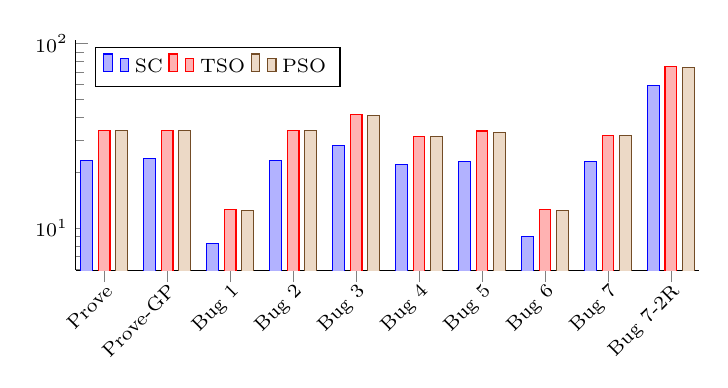
\begin{tikzpicture}
\scriptsize
\begin{axis}[
  ybar,
  bar width=0.15cm,
  height=4.5cm,
  width=9.5cm,
  axis lines*=left, % remove lines in the background
  ymode=log,
  %ylabel=Maximum memory consumption (gigabytes),
  symbolic x coords={Prove, Prove-GP, Bug 1, Bug 2, Bug 3, 
                     Bug 4, Bug 5, Bug 6, Bug 7, Bug 7-2R,
                    },
  xtick=data,
  %nodes near coords, % numbers displayed above the bars
  %every node near coord/.append style={font=\small, rotate=90, anchor=west},
  xticklabel style={
    inner sep=0pt,
    anchor=north east,
    rotate=45
  },
  %enlargelimits=0.15,
  enlarge y limits=0.15, % space relative to the height of the plot
  enlarge x limits=0.05, % space relative to the width of the plot
  legend style={
    %anchor=north, at={(0.5, -0.9)}, % legend location
    legend pos=north west,
    legend columns=-1,
    font=\scriptsize},
]

\addplot % SC
  coordinates {(Prove, 23.27) (Prove-GP, 23.90)
               (Bug 1, 8.24) (Bug 2, 23.26) (Bug 3, 28.04)
               (Bug 4, 22.18) (Bug 5, 23.02) (Bug 6, 9.03)
               (Bug 7, 22.87) (Bug 7-2R, 59.07)
              };

\addplot % TSO 
  coordinates {(Prove, 34.00) (Prove-GP, 34.00)
               (Bug 1, 12.60) (Bug 2, 34.01) (Bug 3, 41.18)
               (Bug 4, 31.49) (Bug 5, 33.65) (Bug 6, 12.59)
               (Bug 7, 31.93) (Bug 7-2R, 74.80)
              };


\addplot % PSO
  coordinates {(Prove, 33.76) (Prove-GP, 33.76)
               (Bug 1, 12.42) (Bug 2, 33.75) (Bug 3, 40.95)
               (Bug 4, 31.27) (Bug 5, 33.04) (Bug 6, 12.44)
               (Bug 7, 31.71) (Bug 7-2R, 74.51)
              };

\legend{SC, TSO, PSO}
\end{axis}
\end{tikzpicture}
